\documentclass{beamer}

\usepackage[textsize=footnotesize]{todonotes}
\usepackage{graphics} % resize table

\usetheme[compress]{Singapore}
\setbeamertemplate{footline}[frame number]
\setbeamercovered{transparent}
\beamertemplatenavigationsymbolsempty
%\setbeamertemplate{navigation symbols}{}

\title{\uppercase{Electric Vehicle X Driving Range Prediction - EV X DRP}}
\subtitle{Relatório de progresso}
%\subtitle{}
\author{
	{\large David P. Coutinho \qquad Artur J. Ferreira} \\
	{\qquad \hspace{-1cm} david.coutinho@isel.pt \qquad arturj@isel.pt} \\
    {\vspace{1cm}}
    {\large David A. S. G. Albuquerque} \\
    {A43566@alunos.isel.pt}
}
\institute
{
	\vspace{0.5cm} \\
	{\normalsize Instituto Superior de Engenharia de Lisboa } \\
}
\date{
	\vspace{-0.75cm}
	Friday, 25 March 2022
}

\usepackage[style=alphabetic]{biblatex}
\addbibresource{bibliography.bib}

\begin{document}

\begin{frame}[t,plain]
    \titlepage
\end{frame}

\begin{frame}
    \frametitle{Outline}
    \tableofcontents
\end{frame}

\section[Introdução]{Introdução}
\subsection[Objetivo]{Objetivo}
\begin{frame}
\frametitle{Introdução - Objetivo}

\begin{itemize}
	\item Cálculo das estimativas de distância de condução restante 
	que um veículo elétrico pode efetuar relativamente ao estado da sua bateria - \textit{eRange}
	\item Aliviar a ansiedade do condutor
\end{itemize}

\begin{figure}[H]
    \begin{center}
        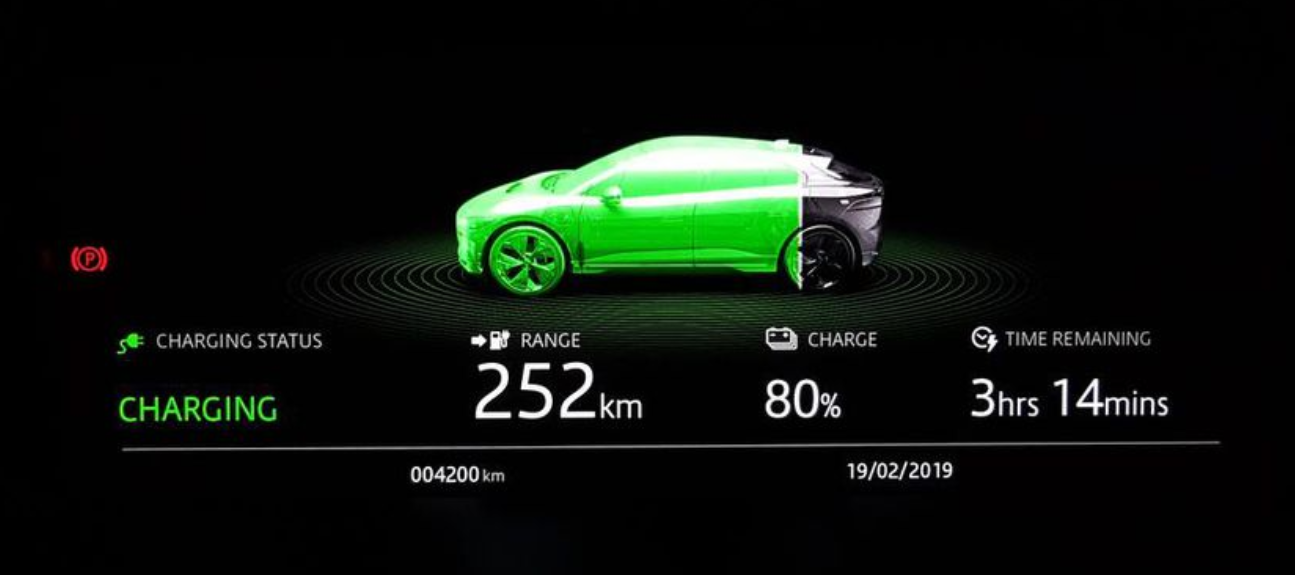
\includegraphics[scale=0.25]{./figures/erange_gauge}
    \end{center}
\end{figure}

\end{frame}


\subsection[Que fatores influenciam o \textit{eRange}?]{Que fatores influenciam o \textit{eRange}?}
\begin{frame}
\frametitle{Introdução - Que fatores influenciam o \textit{eRange}?}

\begin{itemize}
	\item SOC (\textit{State of charge}) - indica o estado de carga da bateria
	\item Estado do ar condicionado / Aquecimento
	\item Condições atmosféricas
	\item Inclinação da estrada
	\item Travagem regenerativa
	\item (entre outros)
\end{itemize}


\end{frame}

\subsection[Formulação do problema]{Formulação do problema}
\begin{frame}
\frametitle{Introdução - Formulação do problema}

\begin{itemize}
	\item Desenvolvimento aplicacional - TODO:
	\begin{itemize}
		\item Uso de inteligência artificial (\textit{machine learning}) para a resolução do problema
		\item Aprendizagem do modelo através de \textit{datasets} contendo os consumos em viagens efetuadas por carros electricos
	\end{itemize}
\end{itemize}

\end{frame}

\subsection[Dificuldades do problema]{Dificuldades do problema}
\begin{frame}
\frametitle{Introdução - Dificuldades do problema}

\begin{itemize}
	\item Escassez de \textit{datasets} para testes de algoritmos
	\item Escolha dos algoritmos de \textit{machine learning}
	\item Dependência de vários fatores aumenta a complexidade do problema
	 \begin{itemize}
			\item Limitado aos fatores existentes nos \textit{datasets}
			\item Seleção de fatores mais relevantes% Reduzir complexidade de algoritmos
		  \end{itemize}
\end{itemize}

\end{frame}

\section[Estado da arte]{Estado da arte}
\subsection[Datasets]{Datasets}
\begin{frame}
\frametitle{Estado da arte - \textit{Datasets}}

\begin{itemize}
	\item \textit{EV Database} (ev-database.org) \footfullcite{onlineEvDatabase}
	\item \textit{VED Dataset} \footfullcite{vedDatasetCleared}
		  \begin{itemize}
			  \item Dados reais de condução de veículos elétricos (2013 Nissan leaf)  
		  \end{itemize}
	\item \textit{Emobpy} \footfullcite{emobpyCleared}
		  \begin{itemize}
			  \item Geração de dados de condução de veículos elétricos
		  \end{itemize}
\end{itemize}

\end{frame}

\subsection[\textit{Datasets} de condução]{Datasets}
\begin{frame}
\frametitle{Estado da arte - \textit{Datasets} de condução}

\begin{table}[]
	\centering
	\resizebox{\textwidth}{!}{%
	\begin{tabular}{c|c|c|}
	\cline{2-3}
														  & VED dataset                                                                                                                                                                  & Emobpy                                                                                              \\ \hline
	\multicolumn{1}{|c|}{Tipo de viagens}                 & Reais                                                                                                                                                                        & Geradas                                                                                             \\ \hline
	\multicolumn{1}{|c|}{Número de viagens}               & 507                                                                                                                                                                          & Infinitas                                                                                           \\ \hline
	\multicolumn{1}{|c|}{Modelos de veículos disponíveis} & 1                                                                                                                                                                            & 102                                                                                                 \\ \hline
	\multicolumn{1}{|c|}{Parâmetros úteis}                & \begin{tabular}[c]{@{}c@{}}velocidade, SOC da bateria,\\ potência do aquecimento,\\ potência do ar condicionado, \\ currente da bateria, \\ voltagem da bateria\end{tabular} & \begin{tabular}[c]{@{}c@{}}distância, consumo,\\ consumo instantâneo,\\ potência média\end{tabular} \\ \hline
	\end{tabular}%
	}
	\end{table}

\end{frame}

\subsection[Implementacoes]{Implementações}
\begin{frame}[label={Implementacoes}]
\frametitle{Estado da arte - Implementações}

\let\oldfootnotesize\footnotesize
\renewcommand*{\footnotesize}{\oldfootnotesize\tiny}

\begin{itemize}
	\item Uso combinado de \textit{Gradient Boosting Regression Trees}
		  \footfullcite{machineLearningERangeGradientBoostRtsCleared};
	\item \textit{Ensemble learning} \footfullcite{eRangeMachineLearningEnsembleCleared} com: 
		  \begin{itemize}
			  \item \textit{Decision Tree };
			  \item \textit{Random Forest};
			  \item \textit{K-Nearest Neighbor}.
		  \end{itemize}
	\item \textit{Self-Organizing Maps}\footfullcite{eRangeMachineLearningGHSOMCleared} 
		  (e híbridos com \textit{Regression Trees} \footfullcite{machineLearningERangeSOMandRtsCleared});
	\item Redes neuronais com \textit{Multiple Linear Regression} 
		  \footfullcite{eRangeMachineLearningNeuralnetworkMLRCleared}.
\end{itemize}

\renewcommand*{\footnotesize}{\oldfootnotesize}

\end{frame}

\section[Trabalho realizado]{Trabalho realizado}
\begin{frame}
\frametitle{Trabalho realizado}

\begin{itemize}
	\item Estudo do problema e soluções existentes
	\item Estudo de \textit{datasets}
	\item Implementação de dois algoritmos para cálculo do \textit{eRange}:
		  \begin{itemize}
			  \item Algoritmo básico ... (TODO) 
			  \item Algoritmo \textit{history-based} \footfullcite{classicEVXCleared2}
		  \end{itemize}
\end{itemize}

\end{frame}

\section[Trabalho futuro]{Trabalho futuro}
\subsection{Objetivos futuros}
\begin{frame}
\frametitle{Trabalho futuro}

\begin{itemize}
	\item Arquitetura de projeto:
		  \begin{itemize}
			  \item Escolha do algoritmo de \textit{machine learning};
		  \end{itemize} 
	\item Implementação do projeto:
		  \begin{itemize}
		      \item Integração do \textit{dataset};
		      \item Implementação do modelo;
		  \end{itemize}
	\item Testes;
	\item Recolha de resultados.
\end{itemize}

\end{frame}

\subsection{Diagrama}
\begin{frame}
\frametitle{Trabalho futuro - Diagrama}

\begin{center}
	\begin{figure}[H]
		\begin{center}
			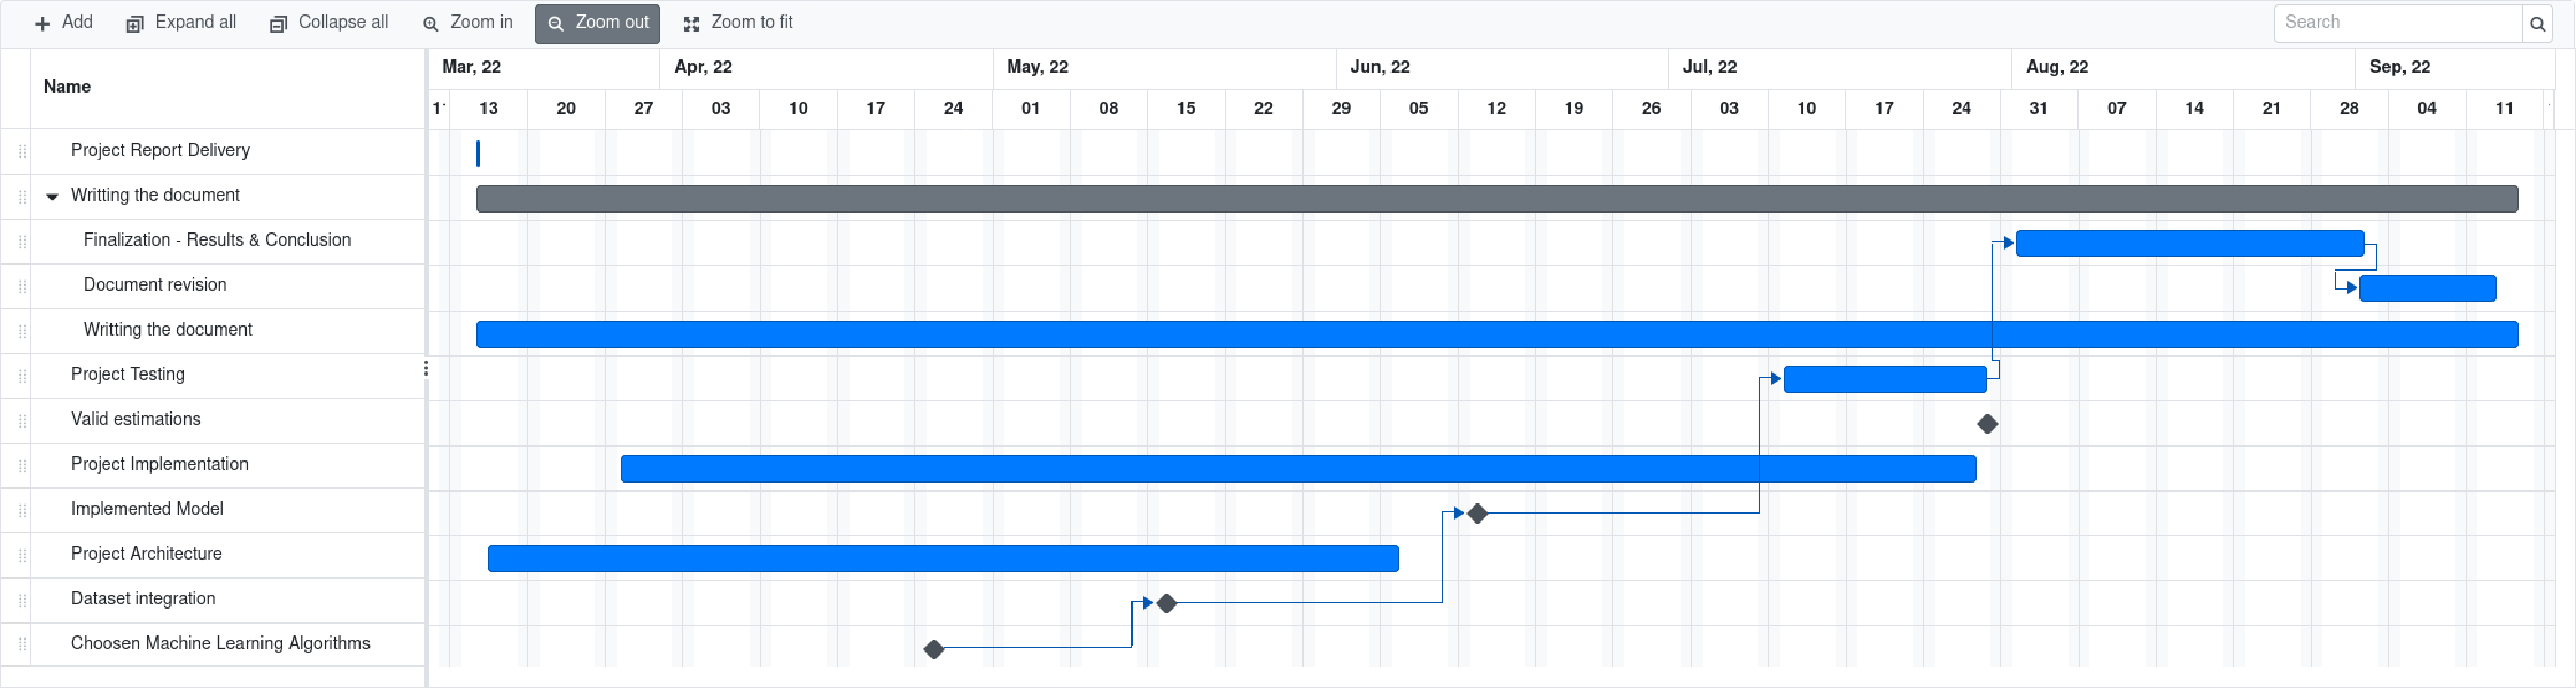
\includegraphics[scale=0.16]{./figures/planning_tiny1.pdf}
		\end{center}
	\end{figure}
\end{center}


\begin{figure}[H]
    \begin{center}
        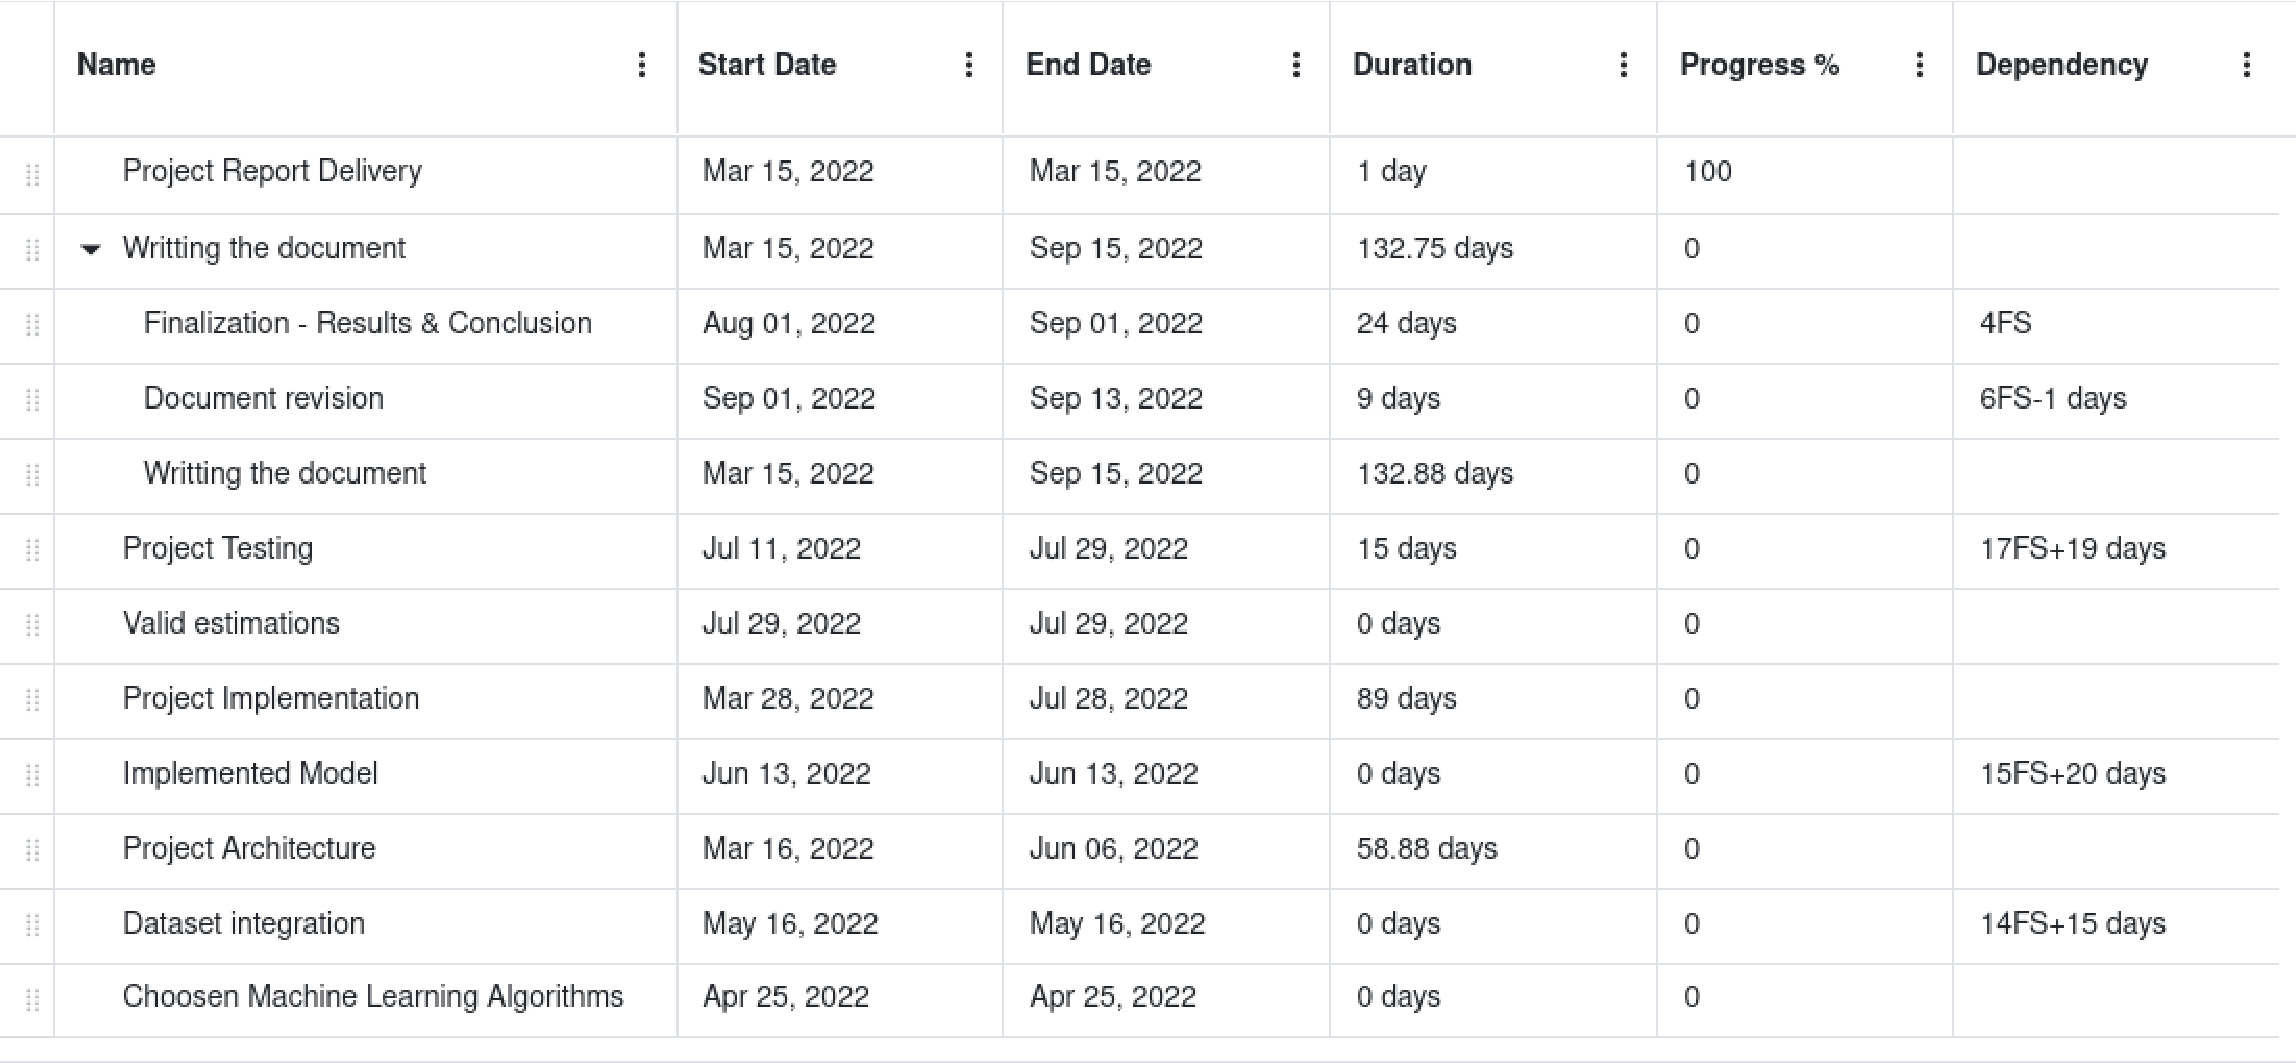
\includegraphics[scale=0.20]{./figures/planning_tiny2.pdf}
    \end{center}
\end{figure}

\end{frame}

\end{document}